In the previous two sections we have discussed multiple benchmarks in two different classes: hand-written benchmarks and randomly generated benchmarks.
We have discussed the advantages and disadvantages of both.
Hand-written benchmarks cost many person-hours to write and maintain, and are usually very limited due to \ac{IP}.
Random benchmarks can overcome the scarcity of hand written ones at the cost of accuracy, they are less realistic and not as useful for assessing how well a method will perform on real use-cases.
There is a third approach that sits in-between the two above, to use machine learning to generate benchmarks with realistic properties.
This section discusses this approach and its limitations.

\subsection{Generative models}
\label{sec:generative}

\begin{figure*}[th]
	\centering
	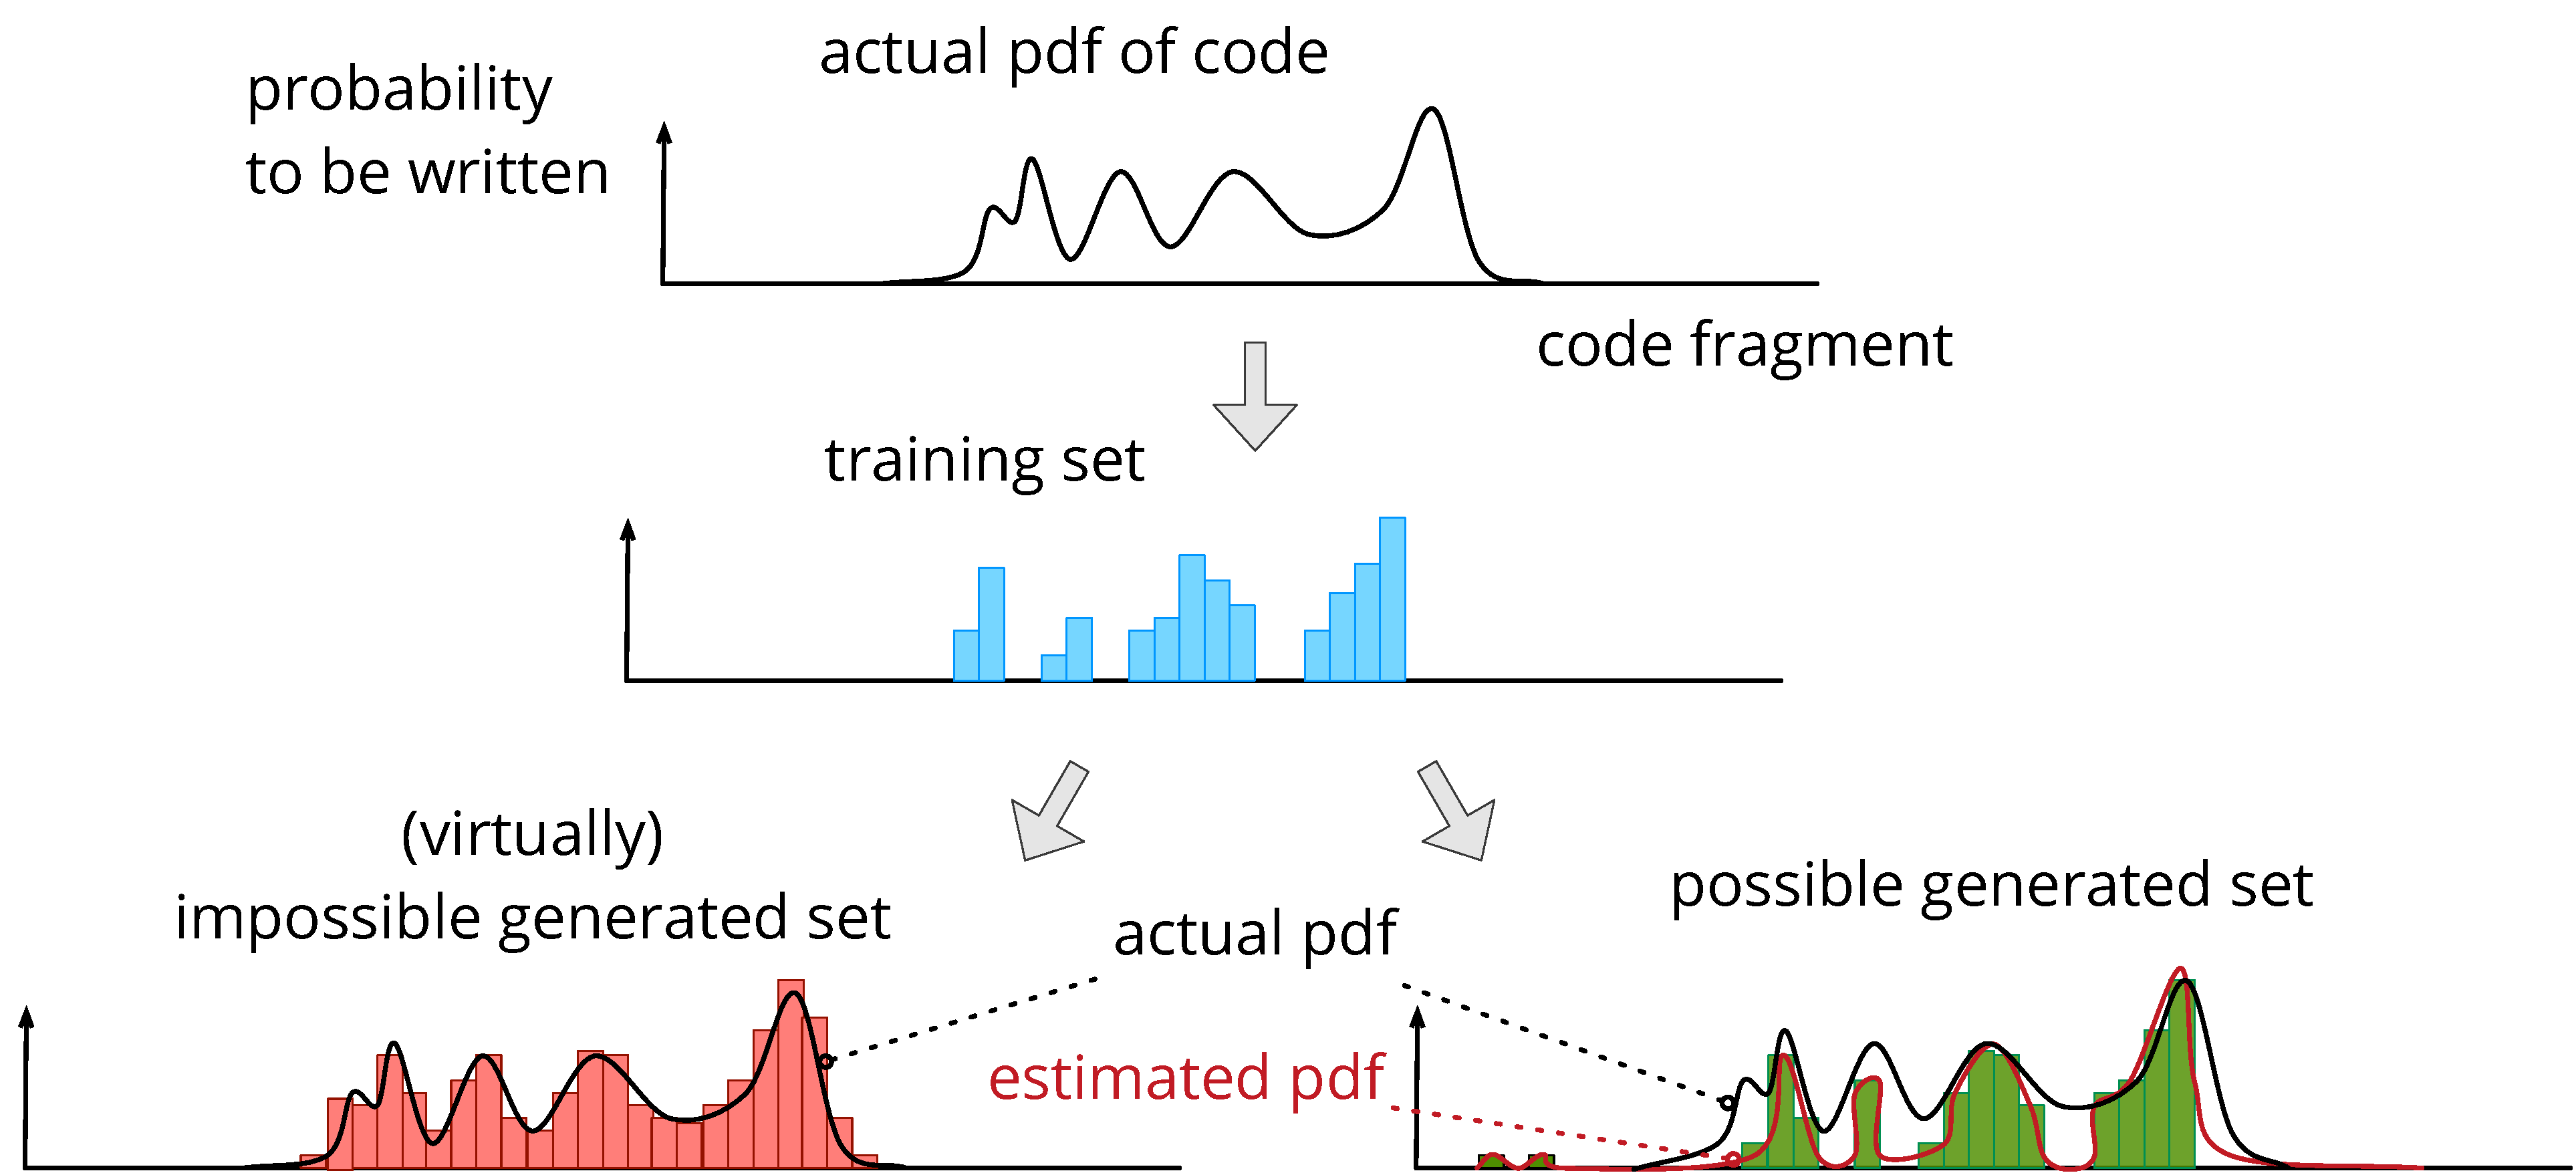
\includegraphics[width=\textwidth]{figures/illustration_histograms_ideal.pdf}
	\caption{An illustration of generative models in the Fischer-Wald setting.}
	\label{fig:histograms}
\end{figure*}

Machine learning models that could generate benchmarks fall under the general term ``generative models''.
There are different classes of generative models, however:
%Let again $p$ be the probability density function describing the probability of a programmer writing a piece of code $\omega \in \Omega$.
\begin{enumerate}
\item \label{fischer-wald} A model in the \textbf{Fischer-Wald setting} is a machine learning model solving the problem of density estimation~\cite{vapnik}. This means finding a probability $p'(t,\alpha_0)$ in a set of probabilities $\{ p'(t,\alpha) \mid \alpha \in \Lambda \}$ parametrized by elements of the parameter set $\Lambda$,
  such that for the risk functional $R(\alpha) = \int -\log(p'(t,\alpha)) dp(t)$, the value of $R(\alpha_0)$ is minimal over all $\alpha \in \Lambda$.
\item \label{conditional-estimation} A \textbf{conditional estimation} model can again mean a solution to a few different problems in different settings. For a random variable $Y$ over code, it estimates either the joint distribution $X \times Y$ or one of the conditional probabilities $p(y \mid X = x)$ or $p(x \mid Y = y)$, where $X$ is the random variable representing a piece of code (i.e. $X(\omega) = \omega$, the identity on $\Omega$)~\cite{vapnik}.

\end{enumerate}

Conditional estimation generative models have plenty of applications.
For example, conditional estimation generative models can be used for code completion tasks, which could even be leveraged to create code that is close to a specified feature vector.
With well-chosen features, this would allow for tools to create other kinds of benchmarks out of, e.g. a representative data set (see Section~\ref{sec:representative}). 
Even more so, this could be used to create domain-specific benchmarks with more samples out of a small domain-specific dataset, by producing code with feature vectors as extracted from the small dataset.
Tuning heuristics and even auto-completion tasks could all be based on conditional estimation models.
The focus of this section is the discussion of using solutions to (\ref{fischer-wald}) for benchmark generation.
This problem is the basis for generative models of code, and solutions to (\ref{conditional-estimation}) are based on or related to it as well.

\subsection{Potential Problems}
\label{sec:potential_problems}
Generative models learn to produce samples similar to those they have seen in the training data. They could then be leveraged to create arbitrarily large benchmark sets.
The problem with this is that, in the ideal case for the Fischer-Wald setting, the code produced by the generative model should be indistinguishable from the training data.
Concretely, it should be code that is also i.i.d. with respect to the (implicit) pdf of code.
If this training set is available, then it can be used instead of the synthesized benchmarks.
Figure~\ref{fig:histograms} illustrates this further.

The theoretical \ac{pdf} depicted represents, again, the probability for a particular program to be written.
To the right the illustration represents a plausible histogram of the code actually present in a training set.
Underneath it, two additional histograms are depicted. To the right, in green, a histogram that is plausibly synthesized by a good generative model trained with the training set.
While it need not be identical to the training set, it should be similar if the generative model has been trained well.
To the left, a histogram is depicted that illustrates a very implausible generated set.
How should the generative model know of the unlikely cases it has not seen, and produce no synthetic code that would never be written by a human?
By the definition in (\ref{fischer-wald}), the closer the histograms are to the depicted pdf, the better are the generative model and training set.

In case we want a ``representative benchmark'', it is thus not clear that a generative model like this is useful.
The programs created by the generative model are i.i.d. with respect to some $p'(t) = p'(t,\alpha_0)$ that is different from $p$.
For estimating $E[\mathcal{P}]$ we get additional accuracy by increasing the number of samples $l$ we use to estimate it.
This additional accuracy, however, could be canceled out by the error in $p'$ (as quantified by, e.g. $R(\alpha_0)$).
Whether this is the case, of course, depends on the concrete problem and errors, and cannot be concluded generally.
We believe, however, that it is probably the case for most instances of the state-of-the-art in generative models of code.
It is likely that with the current state of generative models, where enough training data is present to train such a model, the raw data should be at least good enough, if not even better than synthetic data from the model.

For the other kinds of benchmark, the situation is less problematic.
If we have a filter to distinguish the types of programs, e.g. one based on vectors of features interesting for the use case, then we can use generative models with these filters to produce benchmark sets of the kinds ``representative coverage benchmark'' and perhaps in some cases even ``fuzzing benchmark'', if the generative models generalize well and are run long enough to produce enough data.

\begin{figure*}[th]
	\centering
	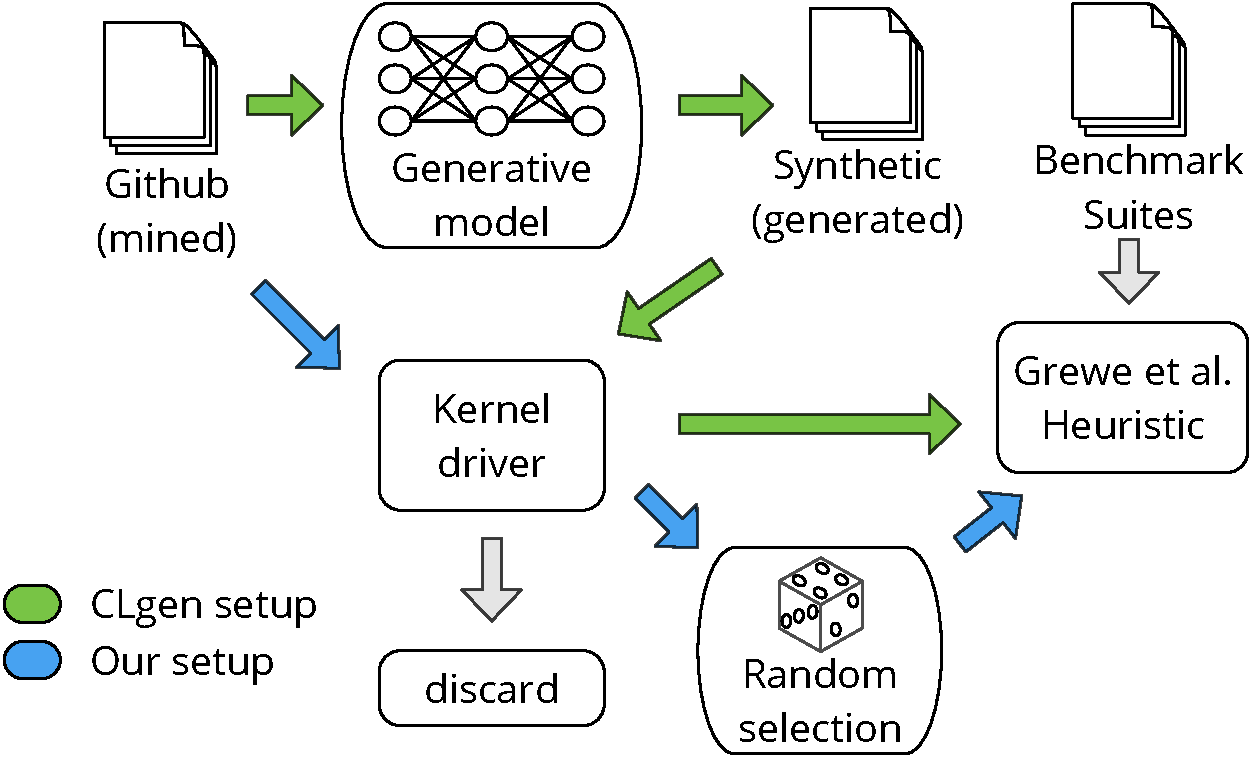
\includegraphics[width=.8\textwidth]{figures/clgen_flow.pdf}
	\caption{The flow of CLGen and our re-evaluation. Reproduced from Figure~1 in~\cite{goens_mapl19}.}
	\label{fig:clgen_flow}
\end{figure*}

We investigated these problems in~\cite{goens_mapl19}, where we re-evaluated the benchmark generation of CLGen~\cite{cummins_cgo17}.
Figure~\ref{fig:clgen_flow} summarizes the flow of CLGen and our re-evaluation.
In the original CLGen setup, the authors of~\cite{cumins_cgo17} mined kernels from Github to train a generative model of code.
The model in CLGen was a character-based model using a \ac{LSTM}\cite{lstm} architecture to learn a character distribution from (normalized) code.
The generative model is then used to generate synthetic benchmarks. A driver ensures they compile and provides input values for the generated benchmarks, which are used together with a set of established benchmark suites to train a heuristic.
The Grewe et al. heuristic~\cite{grewe_cgo2013} trained from these benchmarks is a machine learning model that decides based on a set of hand-designed code features whether to execute an OpenCL kernel in a \acsu{CPU} or the \acsu{GPU}. 
Our setup~\cite{goens_mapl19} takes the alternative route of foregoing the generative model, and using the mined github kernels instead of the synthetic benchmarks.

\begin{figure}[h]
	\centering
\resizebox{0.95\textwidth}{!}{
     \input{generated/clgen_accuracy}
     }
   \caption{Accuracy obtained by the heuristic for the different datasets in the setup. Adapted from Figure~2 of~\cite{goens_mapl19}.}
   \label{fig:clgen_accuracy}
\end{figure}

Figure~\ref{fig:clgen_accuracy} shows box plots comparing the accuracy obtained by the heuristic using the different datasets in both scenarios.
In all cases, one of the benchmarks was excluded from the training dataset and used as test set. We repeated the experiment for all benchmark suites as test set.
For the Github dataset we select a subset of the same size ($1000$) as the CLGen dataset used, which is part of the artifact of~\cite{cummins_cgo17}.
We repeat a random selection of a subset of the Github data $100$ times and report the median accuracy obtained this way, to control for the size of the dataset.
We also consider both the enhanced datasets as in the original work~\cite{cummins_cgo17}, namely the benchmarks enhanced with the CLGen kernels and alternatively enhanced by the original mined Github kernels.
Finally we also consider using each dataset on its own for training, to help the comparison between the usefulness of the Github kernels and the generated CLGen kernels. 
It is obvious that the kernels generated by CLGen are not as useful for training as are the original Github kernels.
We also empirically showed that adding more kernels did not help (see~\cite{goens_mapl19}).
We believe the problem is that the generated kernels are not \emph{representative}.
They are not as useful for maximizing $E[\mathcal{P}]$ as outlined above, $\mathcal{P}$ being the accuracy of the \ac{CPU}/\ac{GPU} mapping.
We have to be careful with the conclusions we can draw from this.
Particularly, upon closer examination (see~\cite{goens_mapl19}), the feature space of the Grewe et al~\cite{grewe_cgo2013} heuristic seems to be rather ill-suited for the task.

\begin{figure}[h]
	\centering
\resizebox{0.95\textwidth}{!}{
     \input{generated/clgen_pca}
     }
   \caption{Smoothed relative frequencies of kernels as function of the first principal component. Adapted from Figure~6 of~\cite{goens_mapl19}.}
   \label{fig:clgen_pca}
\end{figure}

Figure~\ref{fig:clgen_pca} shows a smoothed estimation of the relative frequencies of kernels. The feature space is obviously not one-dimensional. We thus project it into one dimension for visualization by making a principal component analysis using all points.
The figure shows the relative frequencies as a function of the first principal component, i.e. the one with the largest eigenvalue (by modulus). 
This figure thus serves to reproduce the intuition of representativeness as illustrated in Figure~\ref{fig:histograms}.
It is very clear that the (feature) space covered by the benchmarks is larger than that covered by the Github kernels. These, in turn, cover more of the feature space than the generated CLGen kernels.
This results are a consistent with an explanation of the results from Figure~\cite{fig:clgen_acuracy} within the formalism as introduced here.
Concretely, considering the formalism of benchmarks as reproducing a particular probability density and considering the task we want to learn as a random variable.
We believe this probabilistic model of benchmarks has the potential to drive research forward in this direction, and we should focus on it in future work.

A clear first conclusion from this re-thinking of the benchmarking model is that we should also question the objective we are measuring in Figure~\ref{fig:clgen_accuracy}.
The accuracy we consider is the accuracy on the established benchmark suites.
While this seems natural, the question is, is it the most useful objective?
In a real-world scenario we will have our own codebase and will want to get the maximal accuracy in our code base.
Good performance in the benchmarks is only useful to us if our code is similar to that on the benchmarks. 

To evaluate this scenario, we took all kernels $91$ from a concrete project, the Freedesktop project\footnote{https://www.freedesktop.org/}, and removed them form the Github dataset.
The choice of the project is arbitrary, the important property being that it has a moderate amount of kernels without significantly reducing the Github dataset to the point we cannot use it.
Using the same methods as above, we assessed the accuracy of training with all seven\footnote{the benchmark suites are: AMD SDK, NPB, NVIDIA SDK, Parboil, Polybench, Rodinia, SHOC} benchmark suites compared to the Github kernels, without the Freedesktop kernels, obviously.
Surprisingly, the heuristic performed significantly better with the Github kernels at $73\%$, compared to the $48\%$ obtained with the established benchmarks.
These results support the thesis that the concept of representativeness is central to benchmarking and models like the one proposed here should be investigated more.

\subsection{Models of Code}

One property of the generative models in CLGen is the way they represent code.
They do so by considering the (normalized) code as a stream of characters that the model learns to predict.
So far in this thesis we have strongly motivated graph-based representations of code, from the dataflow graphs even to the closely-related level graphs.
It is certainly not a new insight that graphs are well-suited to represent code in its non-linearity.
Compiler construction in general is based on multiple graphs, like the syntax trees or \acp{CDFG}.

Based on this we investigated graph-based representations of code for machine learning, specifically focusing on compilers~\cite{brauckman_cc20}.
Graph models in machine learning are an emerging field, with \acp{GNN}~\cite{gnn} being successful in multiple reasoning tasks.
In the context of programming language models, \acp{GNN} have also been very successful~\cite{allamanis2017learning,cummins_programl,ye2020deep,paliwal2020graph}.
These models use a iterative message-passing semantics to learn the dependencies from adjacent nodes in a graph. 
We designed code representations based on two graph representations of code common in compilers~\cite{brauckmann_cc20}, \acp{CDFG} and \acp{AST}, as well as a general framework for investigating these kinds of code representations~\cite{brauckmann_fdl20}.
Details about the machine learning architecture are beyond the scope of this thesis, here we just discuss the graph-based models and how they expose their semantics.

\begin{figure}[h]
	\centering
\resizebox{0.95\textwidth}{!}{
     \input{generated/graph_representations_code}
     }
   \caption{A comparison of the accuracy of multiple machine learning methods for the \ac{CPU}/\ac{GPU} classification of OpenCL kernels. Adapted from Figure~12 of~\cite{brauckman_cc20}.}
   \label{fig:graph_representations_code}
\end{figure}

To test the different compiler-based graph representations of code, we trained~\cite{brauckman_cc20} multiple deep learning models for the OpenCL \ac{CPU}/\ac{GPU} classification task described above.
Figure~\ref{fig:graph_representations_code} shows a comparison of the accuracy of the different graph-based models.
The baseline model by Grewe et al.~\cite{grewe_cgo2013} is the same baseline model from above.
Additionally, we compare with two state-of-the-art deep learning models for this task, DeepTune~\cite{cummins_pact17} and inst2vec~\cite{inst2vec}.
The graph-based models we evaluate are a control flow graph (CFG), and \acf{CDFG}, enhanced with multiple edge annotations, for data dependencies of the return values of function calls (CALL) and store-load memory dependencies (MEM).

The graph shows two distinct evaluation setups.
The first is the random split setup, which is the same one used by~\cite{cummins_pact17,benun_neurips18}.
It joins all seven benchmark suites investigated into a large set of kernels and randomly splits it into $10$ disjoint subsets.
Each of the disjoint subsets is then used as the testing set, training with all other nine.
We report the geometric means of the accuracy~\cite{fleming1986gmean}.

A potential problem with the random split setup is that it mixes kernels from the same benchmark, which are likely to be more similar. 
This goes back to the representativeness argument for the Freedesktop evaluation above.
A random split assumes a more representative benchmark for training.
To investigate how this affects the algorithms, we change the split to also test how they generalize across benchmark suites.
Instead of random disjoint subsets of equal sizes, we split the kernels for test/training according to the benchmark suites.
One suite is used for testing, all others for training, and we again report the geometric mean of the accuracy.
This is the second setup, the grouped split.

The results in Figure~\ref{fig:graph_representations_code} show that graph-based models generally achieved better accuracy than sequence-based ones.
This is not surprising, as it has been discussed that they are better at exposing the non-linear structure of code.
Also not surprising is that all models do worse in the grouped split, when forced to generalize across benchmark suites.
However, it is worth noting that the \ac{CDFG}-based representations performed better on the random split, and the \ac{AST}-based representations performed better on the grouped split.
A \ac{CDFG} is at a level of abstraction closer to the machine than an \ac{AST}, which is closer to the code itself as written by a human.
In this light, it is not surprising that a \ac{CDFG}-based representation was better at learning with a more representative benchmark in the random split.
The problem in that case is more related to the execution of code on a \ac{CPU} or a \ac{GPU}, whereas on the grouped split, understanding the semantics of the code is more important for predicting how it might fare.

In this section we have seen how graph-based representations and the level of abstraction are important, as well as how we should pay closer attention to the representativeness of a benchmark.
A natural question at this stage is whether this insight can be used to improve generative models and generate better, more representative benchmarks.
For this we also need graph-based generative models, which have received less attention than \acp{GNN} in inference.
The graph generative model of~\cite{li2018learning} that works by generating sequences that construct the graph.
While this allows us to create graphs representing code, the sequential structure of the generative sequences still pose some problems.
This model is also very generic, which it easy to generate invalid code graphs, just the same that CLGen can generate invalid code.
In his Diploma Thesis, which I supervised, Alexander Brauckmann managed to generate more valid code samples than CLGen~\cite{Brauckmann-diplom20} (up to 88\%, compared to 38\% for CLGen).
In a related effort, Alexander Thierfelder designed a domain-specific extension to the model of~\cite{li2018learning}, aiming to generate LLVM-based graphs that are correct by construction~\cite{Thierfelder-master20}.
The LLVM language is complex, and we could unfortunately not design a generative model where the graphs are correct by construction, but we could capture most of the LLVM semantics in the model.
Graph-based models of code are a promising direction for future work, which could allow us to generate representative benchmarks, among others~\cite{leather_fdl20}.